\documentclass[twocolumn]{aastex631}
\usepackage{tikz, mathtools}
\usetikzlibrary{shapes.geometric, arrows,arrows.meta,positioning,quotes,automata,decorations.text}
\usepackage{graphicx, xcolor, wrapfig}

\begin{document}

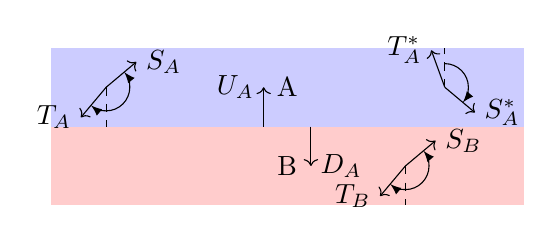
\begin{tikzpicture}
  % Layer A
  \fill[blue!20] (0,0) rectangle (6,1);
  \fill[red!20] (0, -1) rectangle (6, 0);
  \node at (3, 0.5) {A};
  \draw[->] (3.3, 0) -- (3.3, -0.5) node[right] {$D_A$};
  \draw[->] (0.7, 0.5) -- +(40:0.5) node[right] {$S_A$};
  \draw[->] (0.7, 0.5) -- +(230:0.5) node[left] {$T_A$};
  \draw[-, dashed] (0.7, 0.5) -- +(-90:0.5) node {};
  \node at (3, -0.5) {B};
  \draw[->] (2.7, 0) --  (2.7,  0.5) node[left] {$U_A$};
  \draw[-latex] (0.7,0.2) arc
  [
      start angle=-90,
      end angle=40,
      x radius=0.3cm,
      y radius =0.3cm
  ] ;
  \draw[-latex] (0.7,0.2) arc
  [
      start angle=-90,
      end angle=-130,
      x radius=0.3cm,
      y radius =0.3cm
  ] ;
  \draw[->] (5.0, 0.5) -- +(-40:0.5) node[right] {$S^*_A$};
  \draw[->] (5.0, 0.5) -- +(110:0.5) node[left] {$T^*_A$};
  \draw[-, dashed] (5.0, 0.5) -- +(90:0.5) node {};
  \draw[-latex] (5.0,0.8) arc
  [
      start angle=90,
      end angle=-40,
      x radius=0.3cm,
      y radius =0.3cm
  ] ;
  \draw[->] (4.5, -0.5) -- +(40:0.5) node[right] {$S_B$};
  \draw[->] (4.5, -0.5) -- +(230:0.5) node[left] {$T_B$};
  \draw[-, dashed] (4.5, -0.5) -- +(-90:0.5) node {};
  \draw[-latex] (4.5,-0.8) arc
  [
      start angle=-90,
      end angle=40,
      x radius=0.3cm,
      y radius =0.3cm
  ] ;
  \draw[-latex] (4.5,-0.8) arc
  [
      start angle=-90,
      end angle=-130,
      x radius=0.3cm,
      y radius =0.3cm
  ] ;
\end{tikzpicture}

\end{document}